\documentclass{beamer}
\mode<presentation>
\usetheme{CambridgeUS}
\usepackage[russian]{babel}
\usepackage[utf8]{inputenc}
\usepackage[T2A]{fontenc}
\usepackage{sansmathaccent}

\usepackage{verbatim}
\usepackage{alltt}

\pdfmapfile{+sansmathaccent.map}
\title[Файловая система]{Операции над файлами в Linux}
\author{Наумов Д.А., доц. каф. КТ}
\date[12.11.2019] {Операционные системы и системное программное обеспечение, 2019}

\begin{document}

%ТИТУЛЬНЫЙ СЛАЙД
\begin{frame}
  \titlepage
\end{frame}
  
%СОДЕРЖАНИЕ ЛЕКЦИИ
\begin{frame}
  \frametitle{Содержание лекции}
  \tableofcontents  
\end{frame}

\section{Операции над файлами}

\subsection{Удаление файла}

\begin{frame}[fragile]{Удаление файла: unlink()}
Для удаления файла служит системный вызов unlink(), объявленный в заголовочном файле unistd.h следующим образом:
\begin{alltt}
int unlink (const char * FNAME);
\end{alltt}
\begin{itemize}
\item Аргумент FNAME — это имя удаляемого файла. 
\item unlink() возвращает 0 при успешном завершении. 
\item В случае ошибки возвращается –1.
\end{itemize}
\end{frame}

\begin{frame}[fragile]{Удаление файла: unlink()}
\begin{alltt}
#include <stdio.h>
#include <unistd.h>

int main (int argc, char ** argv)
\{
  if (argc < 2) return 1;
  
  if (unlink (argv[1]) == -1) \{
    fprintf (stderr, "Cannot unlink file (\%s)", argv[1]);
    return 1;
  \}
  
  return 0;
\}
\end{alltt}
\end{frame}

\begin{frame}
\begin{block}{Файл}
комплексное понятие, состоящее из следующих компонентов:
\begin{itemize}
\item данные (data);
\item индексы (inodes);
\item ссылки (links).
\end{itemize}
\end{block}
\begin{block}{Индексы}
специальные ячейки памяти, зарезервированные файловой системой для разделения данных на файлы. 
\end{block}
\begin{itemize}
\item Каждый индекс имеет уникальный (в рамках данной файловой системы) номер.
\item Индексы содержат информацию о том, в каких блоках файловой системы хранятся данные конкретного файла. 
\item В индексах содержатся сведения о дате и времени открытия и модификации файла. 
\item Сылка - имя индексного узла файловой системы. 
\end{itemize}
\end{frame}

\begin{frame}[fragile]{Индексы}
Программа ls, вызванная с флагом -i, позволяет увидеть номер индексного узла, на который указывает ссылка:
\begin{alltt}
\$ mkdir idemo
\$ cd idemo
\$ touch file1
\$ touch file2
\$ ls -i

952139 file1 
952141 file2
\end{alltt}
\begin{itemize}
\item file1 — это ссылка на индекс с номером 952139 
\item file2 указывает на другой индексный узел с номером 952141
\end{itemize}
\end{frame}

\begin{frame}[fragile]{Индексы}
Продолжим:
\begin{alltt}
\$ ln -s file1 symlnkf1
\$ ls -i

952139 file1 
952141 file2 
952190 symlnkf1
\end{alltt}
\begin{itemize}
\item символическая ссылка является также ссылкой на индекс с номером 952190
\item символические ссылки указывают не на индекс, а на имя файла
\end{itemize}
\end{frame}

\begin{frame}[fragile]{Индексы}
Теперь воспользуемся командой ln без флага -s:
\begin{alltt}
\$ ln file1 hardfile1
\$ ls -i

952139 file1 952141 file2 952139 hardfile1 952190 symlnkf1
\end{alltt}
\begin{itemize}
\item hardfile1 является жесткой ссылкой на файл file1. Вывод команды ls
показывает, что file1 и hardfile1 указывают на один и тот же индекс с номером 952139. 
\item жесткие ссылки (в отличие от символических) не носят подчиненный характер. file1 и hardfile1 — это полноценные ссылки на один и тот же индексный узел.
\end{itemize}
\end{frame}

\begin{frame}[fragile]{Индексы}
Если две ссылки указывают на один и тот же индекс, то можно сказать, что они имеют доступ к одним и тем же данным:
\begin{alltt}
\$ echo hello > file1
\$ cat hardfile1
hello
\end{alltt}
Индексы являются промежуточным звеном, связывающим ссылку с данными на блочном устройстве. 
\end{frame}

\begin{frame}[fragile]{Команда rm}
Программа rm работает следующим образом:
\begin{itemize}
\item если удаляемый файл является последней ссылкой на соответствующий индексный узел в файловой системе, то данные и индекс освобождаются;
\item если в файловой системе еще остались ссылки на соответствующий индексный узел, то удаляется только ссылка.
\end{itemize}
\begin{alltt}
\$ rm file1
\$ cat hardfile1
hello
\end{alltt}
Теперь обратите внимание на вывод программы ls с флагом -l:
\begin{alltt}
\$ ls -l
-rw-r--r-- 1 kt kt 0 2011-05-07 10:00 file2
-rw-r--r-- 1 kt kt 6 2011-05-07 10:00 hardfile1
lrwxrwxrwx 1 kt kt 5 2011-05-07 10:00 symlnkf1 -> file1
\end{alltt}
\end{frame}

\begin{frame}[fragile]{Команда rm}
Символическая ссылка symlnkf1 по-прежнему указывает на файл file1, которого уже не существует:
\begin{alltt}
\$ cat symlnkf1
cat: symlnkf1: No such file or directory
\end{alltt}
Числа во втором столбце вывода программы ls - счетчики ссылок на соответствующие индексные узлы.
\begin{alltt}
\$ ls -l
-rw-r--r-- 2 kt kt 0 2011-05-07 10:00 file2
-rw-r--r-- 1 kt kt 6 2011-05-07 10:00 hardfile1
-rw-r--r-- 2 kt kt 0 2011-05-07 10:00 hardfile2
lrwxrwxrwx 1 kt kt 5 2011-05-07 10:00 symlnkf1 -> file1
\end{alltt}
\end{frame}

\begin{frame}[fragile]{Команда df}
Если вызвать команду df с флагом -i, то на экран будет выведена информация по индексным узлам смонтированных файловых систем:
\begin{alltt}
\$ df -i

Filesystem Inodes IUsed IFree IUse\% Mounted on
/dev/sda6 1311552 264492 1047060 21\% /
udev 96028 487 95541 1\% /dev
/dev/sda1 66264 58 66206 1\% /boot
/dev/sda7 3407872 149600 3258272 5\% /home
\end{alltt}
В файловых системах может присутствовать ограниченное число индексов (столбец Inodes). Столбец IUsed показывает число используемых индексов, а в столбце IFree содержится число свободных индексных узлов файловой системы
\end{frame}

\begin{frame}[fragile]{Команда df}
Каждый раз при создании файла в файловой системе выделяется индекс:
\begin{alltt}
\$ df -i .
Filesystem Inodes IUsed IFree IUse\% Mounted on
/dev/sda7 3407872 149586 3258286 5\% /home

\$ touch file3
\$ df -i .

Filesystem Inodes IUsed IFree IUse\% Mounted on
/dev/sda7 3407872 149587 3258285 5\% /home
\end{alltt}
\end{frame}

\begin{frame}[fragile]{Команда df}
Создание жесткой ссылки не приводит к появлению в файловой системе нового
индекса:
\begin{alltt}
\$ df -i .
Filesystem Inodes IUsed IFree IUse\% Mounted on
/dev/sda7 3407872 149587 3258285 5\% /home

\$ ln file3 hardfile3
\$ df -i .
Filesystem Inodes IUsed IFree IUse\% Mounted on
/dev/sda7 3407872 149587 3258285 5\% /home
\end{alltt}
\end{frame}

\begin{frame}[fragile]{Пример statvfsinode.c}
В рассматриваемом ранее примере программа использовала функцию statvfs() для вывода информации о смонтированных файловых системах. 

Структура statvfs содержит также следующие поля, которые мы не рассматривали:
\begin{itemize}
\item f\_files — общее число индексов для данной файловой системы;
\item f\_free — число свободных индексов файловой системы;
\item f\_favail — число доступных индексов в файловой системе.
\end{itemize}
\end{frame}

\begin{frame}[fragile]{Пример statinode.c}
Структура stat содержит еще одно поле st\_ino, в котором находится номер индексного узла, на который ссылается файл.
\begin{figure}[h]
\centering
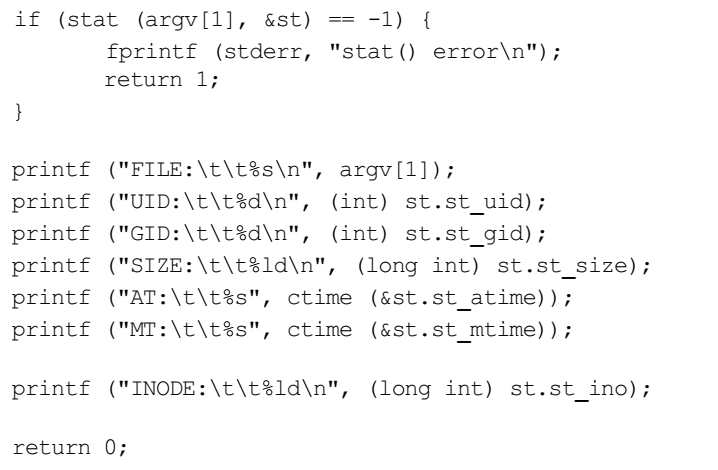
\includegraphics[scale=0.5]{images/lec10-pic01.png}
\end{figure}
\end{frame}

\begin{frame}[fragile]
Cистемный вызов unlink() (unlink2.c) удаляет ссылку на индексный узел. Если эта ссылка была последней, то индекс освобождается.
\begin{alltt}
\$ touch file1
\$ ln file1 file2
\$ ls -i file1 file2
1048740 file1 1048740 file2
\$ ./unlink2 file1
\$ ls file1
/bin/ls: file1: No such file or directory
\$ cat file2
Hello World
\end{alltt}
Над открытым файлом можно успешно осуществлять операции ввода-вывода, даже если последняя ссылка на этот файл удалена:
\begin{alltt}
\$ ./unlink2 file2
\$ ls file2
/bin/ls: file2: No such file or directory
\end{alltt}
\end{frame}

\subsection{Перемещение файла}

\begin{frame}[fragile]{Перемещение файлов}
Системный вызов rename() позволяет переименовывать или перемещать файл в
пределах одной файловой системы.
\begin{alltt}
int rename (const char * OLDF, const char * NEWF);
\end{alltt}
\begin{itemize}
\item При успешном завершении rename() возвращает 0. 
\item В случае ошибки возвращается –1
\end{itemize}
Пример (rename1.c):
\begin{figure}[h]
\centering
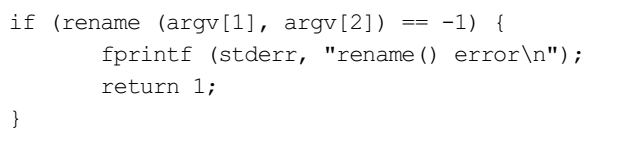
\includegraphics[scale=0.6]{images/lec10-pic02.png}
\end{figure}
\end{frame}

\begin{frame}[fragile]{Перемещение файлов: rename2.c}
Теперь проведем небольшой эксперимент:
\begin{alltt}
\$ touch file1
\$ cat file1
\$ ./rename2 file1 file2
\$ ls file1
/bin/ls: file1: No such file or directory
\$ cat file2
Hello World
\end{alltt}
Перемещение открытого файла никак не отражается на операциях ввода-вывода.
\end{frame}

\subsection{Создание ссылок}

\begin{frame}[fragile]{Создание ссылок}
Ссылки в файловой системе Linux бывают двух типов:
\begin{itemize}
\item символические ссылки (symbolic links);
\item жесткие (прямые) ссылки (hard links).
\end{itemize}
В распоряжении программиста имеются следующие системные вызовы:
\begin{alltt}
int link (const char * FROM, const char * TO);
int symlink (const char * FROM, const char * TO);
\end{alltt}
Оба вызова возвращают 0 при успешном завершении и –1, если произошла ошибка.
Примеры: 
\begin{itemize}
\item linkdemo.c
\item symlinkdemo.c
\end{itemize}
\end{frame}

\subsection{Создание и удаление каталогов}

\begin{frame}[fragile]{Создание каталога}
Для создания каталога используется системный вызов mkdir():
\begin{alltt}
int mkdir (const char * NAME, mode_t MODE)
\end{alltt}
Системный вызов mkdir() создает каталог с именем NAME и режимом MODE. При
успешном завершении mkdir() возвращает 0. В случае ошибки возвращается –1.
Примеры: 
\begin{itemize}
\item mkdir1.c
\item mkdir2.c
\end{itemize}
\end{frame}

\begin{frame}[fragile]{Создание каталога}
Программа mkdir работает не так, как мы ожидали::
\begin{alltt}
\$ ./mkdir2 mydir
\$ ls -l | grep mydir
drwxr-xr-x 2 kt kt 4096 2011-05-07 10:09 mydir
\end{alltt}
В системный вызов mkdir() передавался аргумент mode, в котором все биты базовых прав доступа установлены в единицу. Но вывод программы ls показывает, что созданный каталог имеет права доступа 0755.
\end{frame}

\begin{frame}[fragile]
К каждому процессу в Linux привязана маска прав доступа, которая наследуется потомком от родительского процесса (аналогично текущему каталогу, окружению и т. п.). 
\begin{block}{Маска прав доступа}
число, представляющее собой набор битов прав доступа, которые никогда не будут устанавливаться для создаваемых процессом файлов или каталогов.
\end{block}
Команда umask позволяет узнать текущую маску прав доступа командной оболочки:
\begin{alltt}
\$ umask
0022
\end{alltt}
Маска прав доступа 0022 разрешает при создании файлов или каталогов устанавливать любые права доступа для владельца, но не разрешает права на запись для группы и остальных пользователей.
\end{frame}

\begin{frame}[fragile]{Маски прав доступа}
Текущий процесс вправе изменять свою копию маски прав доступа:
\begin{alltt}
\$ umask 0044
\$ umask
0044
\end{alltt}
Дочерние процессы наследуют копию маски прав доступа родительского процесса:
\begin{alltt}
\$ umask 000
\$ umask
0000
\$ bash
\$ umask
0000
\$ exit
exit
\end{alltt}
\end{frame}

\begin{frame}[fragile]{Создание каталога}
Попробуем запустить программу mkdir2 с измененной маской прав доступа оболочки:
\begin{alltt}
\$ umask 0000
\$ umask
0000
\$ ./mkdir2 mydir
\$ ls -l | grep mydir
drwxrwxrwx 2 kt kt 4096 2011-05-07 10:15 mydir
\end{alltt}
\end{frame}

\begin{frame}[fragile]{Системный вызов umask()}
Программа может изменить маску прав доступа текущего процесса при помощи
системного вызова umask():
\begin{alltt}
mode_t umask (mode_t MASK);
\end{alltt}
Этот системный вызов изменяет текущую маску прав доступа и возвращает предыдущее значение маски.
Примеры: 
\begin{itemize}
\item mkdir3.c
\end{itemize}
\begin{alltt}
\$ umask 0022
\$ umask
0022
\$ ./mkdir3 mydir
\$ ls -l | grep mydir
drwxrwxrwx 2 kt kt 4096 2011-05-07 10:17 mydir
\end{alltt}
\end{frame}

\begin{frame}[fragile]{Создание каталога}
Пример создания каталога с "липким битом":  
\begin{itemize}
\item mkdir4.c
\end{itemize}
\begin{alltt}
\$ ./mkdir4 mydir
\$ ls -l | grep mydir
drwxrwxrwt 2 kt kt 4096 2011-05-07 10:20 mydir
\end{alltt}
\end{frame}

\begin{frame}[fragile]{Удаление каталога}
Для удаления каталога служит системный вызов rmdir():
\begin{alltt}
int rmdir (const char * DIR)
\end{alltt}
\begin{itemize}
\item Аргумент DIR — это имя (путь) к каталогу, который следует удалить.
\item При успешном завершении rmdir() возвращает 0. В случае ошибки возвращается –1. 
\end{itemize}
Пример: 
\begin{itemize}
\item rmdirdemo.c
\end{itemize}
Системный вызов rmdir() удаляет только пустые каталоги. Если каталог не пуст, то rmdir() завершится неудачей.
\end{frame}

%\section{Права доступа}


\end{document} 